\documentclass[12pt]{article}

\newlength\tindent
\setlength{\tindent}{\parindent}
\setlength{\parindent}{0pt}
\renewcommand{\indent}{\hspace*{\tindent}}

%% packages
\usepackage{enumerate}
\usepackage{listings}
\usepackage{amsmath}
\usepackage{multicol}
\usepackage{caption}
\usepackage{subcaption}
\usepackage[a4paper,margin=2cm]{geometry}
% \usepackage[english, norsk]{babel}
\usepackage{fancyhdr}
\usepackage{pdfpages}
\usepackage{lastpage}
% \usepackage[demo]{graphicx}
\usepackage{graphicx}
\graphicspath{ {.} }

%Framed image panel
\newcommand\FramedImage[2][]{%
  \setlength\fboxsep{1pt}% change according to needs
  \setlength\fboxrule{3pt}%
  \noindent\fbox{%
    \begin{minipage}[c][\dimexpr.3\textheight-1.5\fboxrule-2\fboxsep\relax][c]{\dimexpr.5\textwidth-1.5\fboxrule-2\fboxsep\relax}
    \centering
    \includegraphics[#1]{#2}
  \end{minipage}}%
}
\newcommand{\FIXME}[1]{{\bfseries FIXME: #1}}
\newcommand{\COMMENT}[2]{{\bfseries COMMENT~(#1): #2}}
\date{}
\begin{document}

% intentionally empty
%\author{Faculty of Mathematics and Natural Sciences}

\title{Additional exercises}

\maketitle 


\section{Random variable parameter estimation}

A discrete random variable $X$ is defined by
  \begin{equation}
    X=
    \begin{cases}
      -20, & prob.=1/3 \\
       30, & prob.=1/2 \\
       10, & prob.=1/6
    \end{cases}
  \end{equation}

\begin{enumerate}[(a)] 
\item find the expected value
\item find the variance
\item find the mode
\item find the coefficient of variation
\end{enumerate}

\section{Normal distribution}
The annual precipitation at a station has a normal distribution with a mean of 100 cm. What is its standard deviation if the probability is 0.1 that it will take on a value greater than 115 cm?


\section{Frequency analysis}
\begin{enumerate}[(a)] 
\item What is the return period? What is Probability of exceedence? What is a design flood?
\item Assume the yearly maximum discharge of a river is a random variable $X$, such that $\ln X$ is normally distributed with a mean of 5, and a standard deviation of 0.5 if X is expressed in m$^3$/s. ($\ln X$ stands for the natural logarithm). A flood arises when yearly maximum discharge is larger than a critical value q.
 \begin{enumerate}[(i)]
 \item If the probability that a q is exceeded in one year is 0.75, what is q?
 \item If the probability that a q is not exceeded in one year is 0.5, what is q?
 \item Calculate the non-exceedence probability of the discharge 100 m3/s
 \item If the return period of a flood is 10 years, what is then the probability of at least 1 flood in 10-year
 \end{enumerate}
\end{enumerate}


\section{Multiple linear regression}
What are the assumptions behind multiple linear regressions?


\section{Confidence intervals}
A sample of 20 random observations produced a mean of 145 and variance of 30. 
\begin{enumerate}[(a)] 
    \item What is the 95\% confidence interval on the mean assuming a normal distribution if 
    \begin{enumerate}[(i)] 
        \item the true variance is unknown and estimated as 30
        \item the true variance is 30
     \end{enumerate}
    \item What is the reason for the difference of results in part (i) and part (ii)?
    \item What is the 95\% confidence interval on the variance?
\end{enumerate}



\section{Hypothesis testing}
Based on two samples with 10 observations each, the following estimates for mean and standard deviations have been obtained:

$\mu_1=44.1$

$\mu_2=50.0$

$\sigma_1=3.3$

$\sigma_2=5.6$


\begin{enumerate}[(a)] 
    \item Test if the estimates for mean and standard deviation are significantly different. Use a significance level of 5\%.
	\item We make two types of errors in hypothesis testing.
    \begin{enumerate}[(i)] 
		\item Explain type I and type II errors.
		\item Explain and illustrate graphically the relation between type I and type II errors.
     \end{enumerate}
\end{enumerate}



\section{Goodness-of-fit testing}
In order to calculate the design flood, you need to know which probability distribution fits your data best. Based on a 35-year record of yearly maximum discharge data from a river station, the following statistics are calculated (with $n = 35$)

Let $Y = \ln Q$ (natural logarithm)

Average: $\bar{Y}=5.257$ 

Standard deviation: $S_Y = 0.686$

The 35 years data are classified into 5 classes as given in the table below.
\begin{table}[h!!]
\begin{tabular}{l|c}
Class & Observed number \\
\hline
$Q \le 100$ & 5 \\
$100<Q \le 150$ & 9 \\
$150<Q \le 200$ & 7 \\
$200<Q \le 300$ & 6 \\
$Q \ge 300$ & 8 \\
\hline
\end{tabular}
\end{table}


\begin{enumerate}[(a)] 
\item Use Chi square method (with significance level of 5\%) to test if the data are log-normally distributed
\item Could the Kolmogorov-Smirnov test also be used to perform the goodness-of-fit test?
\end{enumerate}


\section{Time series analysis}
A 7-year time series of annual measurements is given as the sequence:\\
110, 88, 51, 64, 39, 23, 10

Perform a trend test of your choice to check if the time series contains a trend. Use a significance level of 5\%.



\section{Time series analysis and stochastic modeling}
Answer the following statements with True if it is always true, otherwise with False.
\begin{enumerate}[(a)] 
\item Most hydrologic processes (time series) are stochastic processes
\item Stochastic process (time series) is stationary 
\item An independent time series is a stationary time series 
\item An independent stationary time series is purely random
\item A Gaussian time series is an independent series
\item A Gaussian time series is a stationary time series
\item A white noise times series is normally distributed
\item If Xt is a log-normally distributed time series, then Xt is symmetric about its mean
\item Markov model (i.e. AR(1) model) is used for an independent stationary time series
\item Markov model (i.e. AR(1) model) is used for a nonstationary time series
\end{enumerate}

\pagebreak

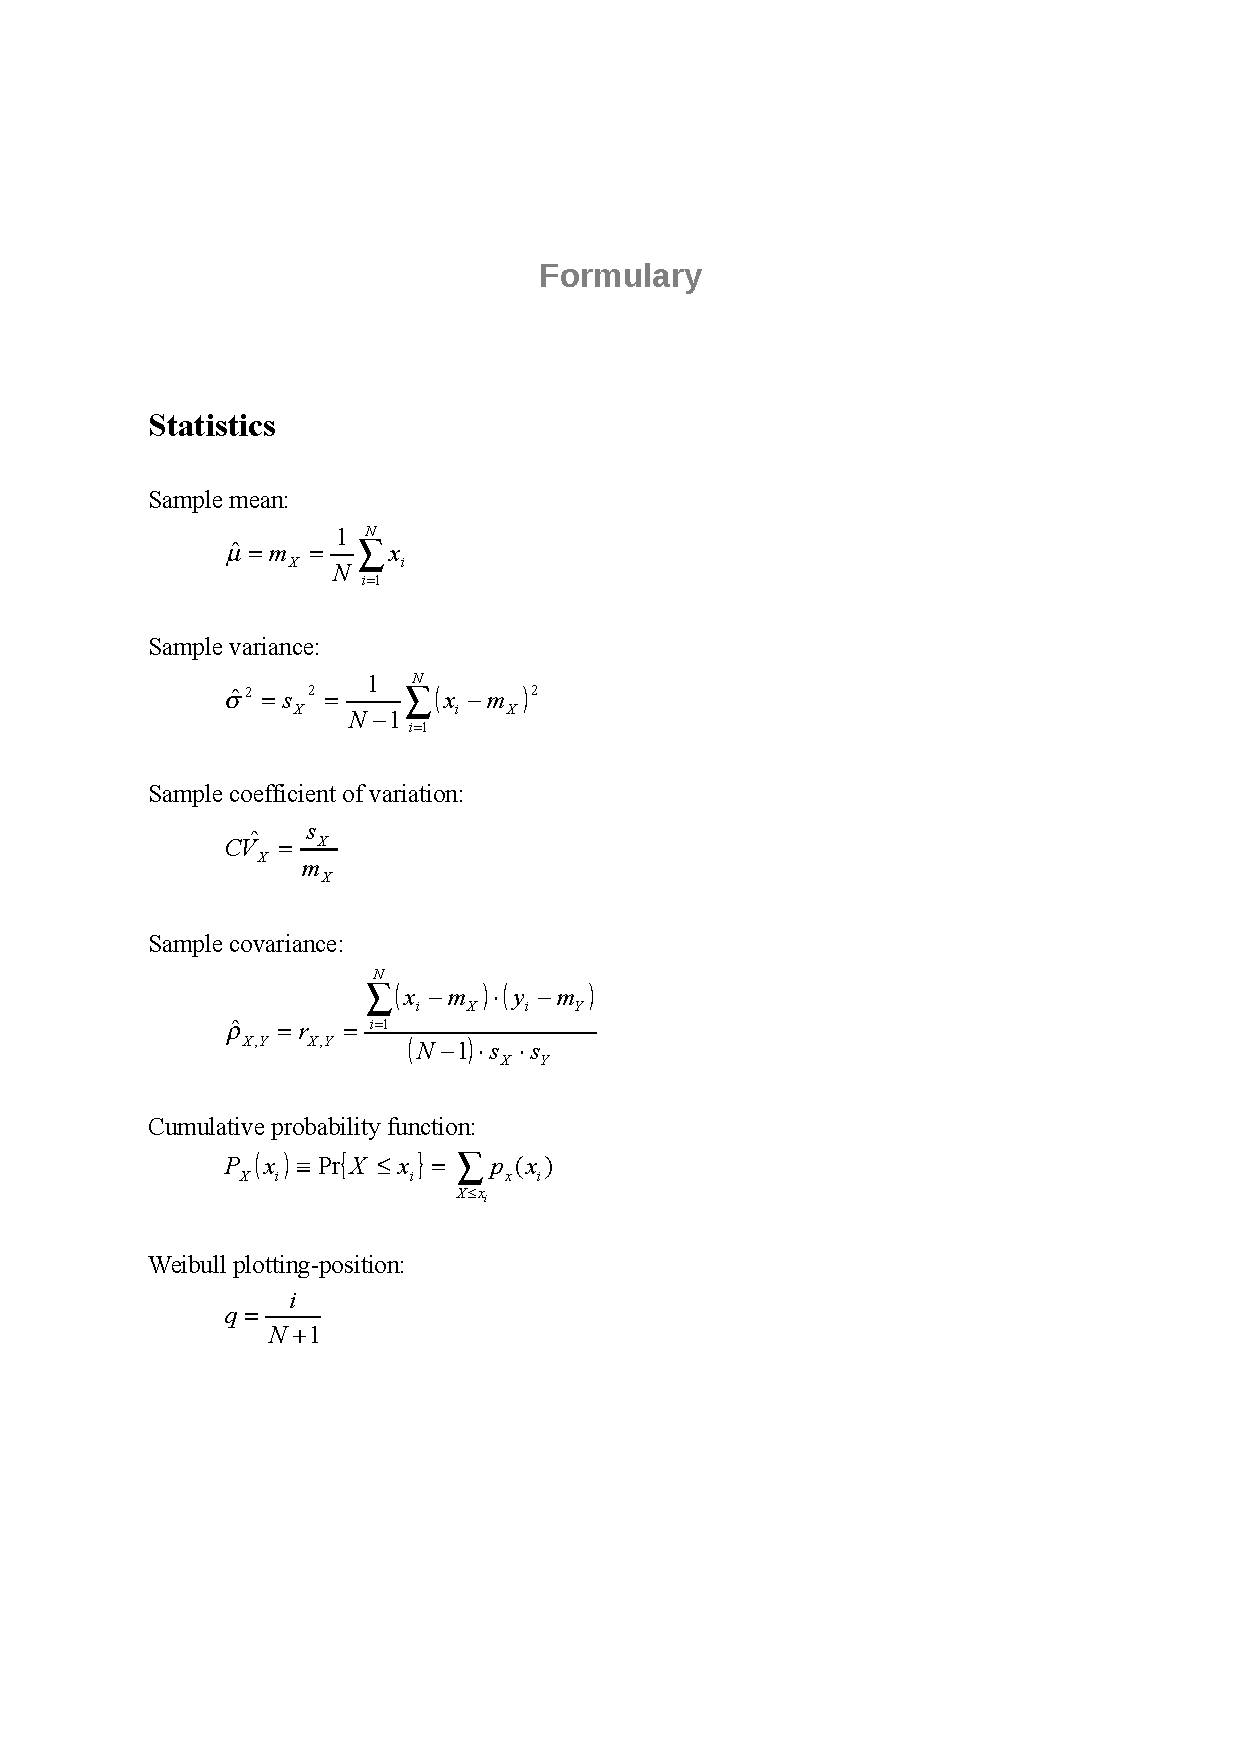
\includepdf[pages={1-12}]{formulary-2017_final.pdf}



\end{document}









